\documentclass[11pt,a4paper]{article}
\usepackage[margin=2cm]{geometry}
\usepackage[T1]{fontenc}
\usepackage[utf8]{inputenc}
\usepackage{hyperref}
\usepackage{xcolor}
\usepackage{listings}
\usepackage{tikz}
\usetikzlibrary{positioning,arrows.meta}
\definecolor{codebg}{RGB}{248,250,252}
\definecolor{codeblue}{RGB}{37,99,235}
\definecolor{codegreen}{RGB}{22,101,52}
\definecolor{codered}{RGB}{185,28,28}
\definecolor{codegray}{RGB}{100,116,139}
\lstdefinelanguage{JavaScript}{morekeywords={const,let,var,async,await,function,try,catch,return,if,else,for,of,require,module,exports},sensitive=true,morecomment=[l]{//},morestring=[b]",morestring=[b]`}
\lstdefinestyle{prokuraCode}{basicstyle=\ttfamily\small,breaklines=true,frame=single,columns=fullflexible,keepspaces=true,showspaces=false,showstringspaces=false,showtabs=false,tabsize=2,numbers=left,numberstyle=\tiny\color{codegray},keywordstyle=\color{codeblue}\bfseries,stringstyle=\color{codered},commentstyle=\color{codegreen},rulecolor=\color{codegray},backgroundcolor=\color{codebg}}
\lstset{style=prokuraCode}
\newcommand{\docheader}[2]{
\begin{titlepage}
\centering
{\Large\bfseries Prokura HoReCa Supply\par}
\vspace{0.4cm}
{\large Dokumentasi Fitur Microservice Final Project\par}
\vspace{0.8cm}
{\large Mata Kuliah: Proyek 2 - Final Project\par}
\vspace{1.2cm}
{\large\bfseries #1\par}
{\large NIM: #2\par}
\vfill
\begin{tabular}{rl}
Program Studi: & Ilmu Komputer\\
Departemen: & Departemen Ilmu Komputer dan Elektronika (DIKE)\\
Fakultas: & FMIPA\\
Universitas: & Universitas Gadjah Mada\\
\end{tabular}
\vfill
\end{titlepage}
}

\begin{document}
\docheader{Indratanaya Budiman}{24/534784/PA/22683}

\section*{Peran}
Owner Order Service. Indratanaya bertanggung jawab pada checkout customer, purchase order, perubahan stok keluar, status PO, dan riwayat pembelian.

\section*{Bukti Microservice}
Order Service berada di \path{prokura-api/src/services/order} dan dapat dijalankan sebagai service tersendiri melalui \texttt{service-host}.

\begin{lstlisting}[language=JavaScript]
const serviceRegistry = {
  catalog: registerCatalogRoutes,
  customer: registerCustomerRoutes,
  inventory: registerInventoryRoutes,
  order: registerOrderRoutes,
  reporting: registerReportingRoutes,
};
\end{lstlisting}

Penjelasan: entry \texttt{order: registerOrderRoutes} menunjukkan Order Service punya boundary terpisah. Pada deployment microservices, Order Service berjalan di port \texttt{5104}, sementara UI tetap memanggil API lewat HTTP.

\section*{Tanggung Jawab Fitur}
\begin{enumerate}
\item Pembelian barang oleh customer.
\item Riwayat pembelian customer.
\end{enumerate}

\section*{Diagram Tabel yang Ditangani}
\begin{center}
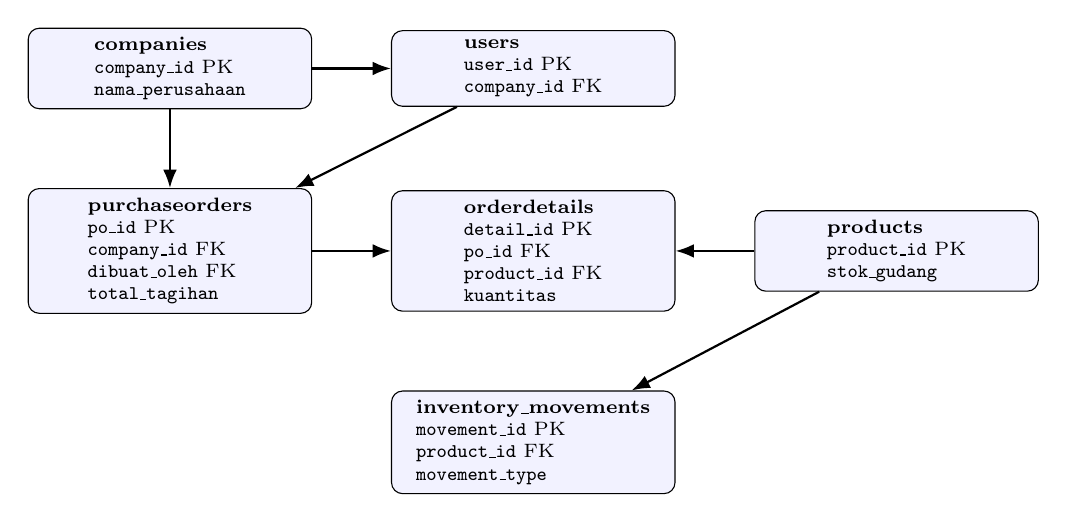
\begin{tikzpicture}[entity/.style={draw, rounded corners, fill=blue!5, align=left, font=\scriptsize, minimum width=3.6cm}, rel/.style={-Latex, thick}]
\node[entity] (companies) {\textbf{companies}\\\texttt{company\_id} PK\\\texttt{nama\_perusahaan}};
\node[entity, right=1.0cm of companies] (users) {\textbf{users}\\\texttt{user\_id} PK\\\texttt{company\_id} FK};
\node[entity, below=1.0cm of companies] (po) {\textbf{purchaseorders}\\\texttt{po\_id} PK\\\texttt{company\_id} FK\\\texttt{dibuat\_oleh} FK\\\texttt{total\_tagihan}};
\node[entity, right=1.0cm of po] (details) {\textbf{orderdetails}\\\texttt{detail\_id} PK\\\texttt{po\_id} FK\\\texttt{product\_id} FK\\\texttt{kuantitas}};
\node[entity, right=1.0cm of details] (products) {\textbf{products}\\\texttt{product\_id} PK\\\texttt{stok\_gudang}};
\node[entity, below=1.0cm of details] (movements) {\textbf{inventory\_movements}\\\texttt{movement\_id} PK\\\texttt{product\_id} FK\\\texttt{movement\_type}};
\draw[rel] (companies) -- (users);
\draw[rel] (companies) -- (po);
\draw[rel] (users) -- (po);
\draw[rel] (po) -- (details);
\draw[rel] (products) -- (details);
\draw[rel] (products) -- (movements);
\end{tikzpicture}
\end{center}

Penjelasan: Order Service membuat \texttt{purchaseorders} dan \texttt{orderdetails}, membaca relasi ke \texttt{companies} dan \texttt{users}, mengurangi \texttt{products.stok\_gudang}, lalu mencatat \texttt{STOCK\_OUT} ke \texttt{inventory\_movements}.

\section*{Lokasi Kode Program dan Penjelasan}
\subsection*{Route checkout order}
Lokasi kode: \path{prokura-api/src/services/order/routes.js}. \texttt{POST /api/orders}: line 46.

\begin{lstlisting}[language=JavaScript]
app.post("/api/orders", async (req, res) => {
  const { company_id, dibuat_oleh, metode_pembayaran, total_tagihan, items } =
    req.body;

  try {
    validateOrderPayload(req.body);
  } catch (error) {
    return res.status(400).json({ success: false, message: error.message });
  }

  const orderTotal = total_tagihan == null ? calculateOrderTotal(items) : Number(total_tagihan);
  const client = await pool.connect();
\end{lstlisting}

Penjelasan: endpoint checkout menerima payload order dari UI, memvalidasi isi payload, lalu menghitung total order jika total belum dikirim. Validasi dilakukan sebelum transaksi database dimulai.

\begin{lstlisting}[language=JavaScript]
await client.query("BEGIN");

for (const item of items) {
  const stock = await lockProductStock(client, item.product_id);
  if (!stock || Number(stock.stok_gudang) < Number(item.kuantitas)) {
    throw new Error(`Stok produk ${item.product_id} tidak cukup`);
  }
}
\end{lstlisting}

Penjelasan: stok tiap produk dikunci dengan \texttt{FOR UPDATE} melalui repository. Ini mencegah dua checkout bersamaan mengambil stok yang sama.

\begin{lstlisting}[language=JavaScript]
const newPoId = await createPurchaseOrder(client, {
  company_id,
  dibuat_oleh,
  metode_pembayaran,
  total_tagihan: orderTotal,
});

for (const item of items) {
  await createOrderDetail(client, newPoId, item);
  await decrementProductStock(client, item);

  await recordInventoryMovement(client, {
    productId: item.product_id,
    movementType: "STOCK_OUT",
    quantity: -Number(item.kuantitas),
    note: `Checkout PO #${newPoId}`,
    referenceType: "ORDER",
    referenceId: newPoId,
  });
}
\end{lstlisting}

Penjelasan: setelah PO dibuat, sistem membuat detail order, mengurangi stok, dan mencatat \texttt{STOCK\_OUT}. Semua langkah berada dalam satu transaksi agar order dan stok tetap konsisten.

\subsection*{Route riwayat dan detail pembelian}
Lokasi kode: \path{prokura-api/src/services/order/routes.js}. \texttt{GET /api/companies/:company\_id/orders}: line 26. \texttt{GET /api/orders/:po\_id}: line 36.

\begin{lstlisting}[language=JavaScript]
app.get("/api/companies/:company_id/orders", async (req, res) => {
  try {
    const { company_id } = req.params;
    const orders = await listCompanyOrders(pool, company_id);
    res.json({ success: true, data: orders });
  } catch (error) {
    sendError(res, error, "Gagal mengambil riwayat PO");
  }
});
\end{lstlisting}

Penjelasan: endpoint ini mengambil daftar PO milik satu perusahaan. Customer dapat melihat riwayat pembelian tanpa mengakses tabel langsung.

\begin{lstlisting}[language=JavaScript]
app.get("/api/orders/:po_id", async (req, res) => {
  try {
    const { po_id } = req.params;
    const details = await listOrderDetails(pool, po_id);
    res.json({ success: true, data: details });
  } catch (error) {
    sendError(res, error, "Gagal mengambil detail PO");
  }
});
\end{lstlisting}

Penjelasan: endpoint ini mengambil item detail dari satu PO sehingga demo bisa menunjukkan barang, kuantitas, harga final, dan subtotal.

\subsection*{SQL repository order}
Lokasi kode: \path{prokura-api/src/services/order/repository.js}. List riwayat customer: line 17. Insert purchase order: line 55. Insert detail order: line 67. Kurangi stok: line 77.

\begin{lstlisting}[language=JavaScript]
const { rows } = await pool.query(
  `
    SELECT po.po_id, po.status_po, po.metode_pembayaran, po.total_tagihan,
           po.tanggal_dipesan, u.nama_lengkap AS pembuat
    FROM purchaseorders po
    JOIN users u ON po.dibuat_oleh = u.user_id
    WHERE po.company_id = $1
    ORDER BY po.tanggal_dipesan DESC
  `,
  [companyId],
);
\end{lstlisting}

Penjelasan: query ini membaca riwayat PO untuk satu perusahaan. Join ke \texttt{users} menampilkan nama pembuat PO.

\begin{lstlisting}[language=JavaScript]
const { rows } = await client.query(
  `
    INSERT INTO purchaseorders (company_id, dibuat_oleh, metode_pembayaran, total_tagihan)
    VALUES ($1, $2, $3, $4)
    RETURNING po_id
  `,
  [order.company_id, order.dibuat_oleh, order.metode_pembayaran, order.total_tagihan],
);
\end{lstlisting}

Penjelasan: query ini membuat header PO dan mengembalikan \texttt{po\_id}. Nilai \texttt{po\_id} dipakai untuk menyimpan detail item.

\begin{lstlisting}[language=JavaScript]
await client.query(
  `
    INSERT INTO orderdetails (po_id, product_id, kuantitas, harga_final)
    VALUES ($1, $2, $3, $4)
  `,
  [poId, item.product_id, item.kuantitas, item.harga_final],
);
\end{lstlisting}

Penjelasan: query ini menyimpan item order. Setiap item berisi produk, kuantitas, dan harga final saat checkout.

\begin{lstlisting}[language=JavaScript]
await client.query(
  `
    UPDATE products
    SET stok_gudang = stok_gudang - $1
    WHERE product_id = $2
  `,
  [item.kuantitas, item.product_id],
);
\end{lstlisting}

Penjelasan: query ini mengurangi stok gudang sesuai kuantitas yang dibeli. Karena sudah ada lock stok sebelumnya, pengurangan stok aman terhadap checkout bersamaan.

\subsection*{UI customer web}
Lokasi kode: \path{prokura-web/app/page.tsx}. Checkout POST order: line 129. Detail PO: line 152. Tombol \texttt{Ajukan Approval}: line 444. Riwayat PO finance: line 460.

\begin{lstlisting}[language=JavaScript]
const res = await fetch(`${API_BASE_URL}/api/orders`, {
  method: "POST",
  headers: { "Content-Type": "application/json" },
  body: JSON.stringify(payload),
});
\end{lstlisting}

Penjelasan: customer web mengirim checkout ke Order Service melalui API gateway. Payload berisi company, user pembuat, metode pembayaran, total tagihan, dan item cart.

\begin{lstlisting}[language=JavaScript]
const res = await fetch(`${API_BASE_URL}/api/orders/${po.po_id}`);
\end{lstlisting}

Penjelasan: saat user melihat detail PO, UI mengambil detail order dari endpoint order, bukan dari database langsung.

\section*{SQL Query Demo dan Penjelasan}
\subsection*{Query 1: buat purchase order}
\begin{lstlisting}[language=SQL]
INSERT INTO purchaseorders (company_id, dibuat_oleh, metode_pembayaran, total_tagihan)
VALUES (1, 1, 'Tempo_30_Hari', 250000)
RETURNING po_id;
\end{lstlisting}
Penjelasan: query ini membuat header PO. \texttt{company\_id} menunjukkan perusahaan pembeli, \texttt{dibuat\_oleh} menunjukkan user, dan \texttt{total\_tagihan} menyimpan nilai transaksi.

\subsection*{Query 2: tambah detail order}
\begin{lstlisting}[language=SQL]
INSERT INTO orderdetails (po_id, product_id, kuantitas, harga_final)
VALUES (currval('purchaseorders_po_id_seq'), 1, 5, 50000);
\end{lstlisting}
Penjelasan: query ini memasukkan item PO untuk produk tertentu. \texttt{currval} memakai \texttt{po\_id} terbaru dari insert purchase order pada sesi yang sama.

\subsection*{Query 3: kurangi stok}
\begin{lstlisting}[language=SQL]
UPDATE products
SET stok_gudang = stok_gudang - 5
WHERE product_id = 1;
\end{lstlisting}
Penjelasan: query ini menurunkan stok produk sesuai kuantitas checkout. Perubahan stok menjadi bukti database berubah akibat pembelian.

\subsection*{Query 4: lihat riwayat pembelian customer}
\begin{lstlisting}[language=SQL]
SELECT po.po_id, po.status_po, po.metode_pembayaran, po.total_tagihan,
       po.tanggal_dipesan, u.nama_lengkap AS pembuat
FROM purchaseorders po
JOIN users u ON po.dibuat_oleh = u.user_id
WHERE po.company_id = 1
ORDER BY po.tanggal_dipesan DESC;
\end{lstlisting}
Penjelasan: query ini menampilkan riwayat PO milik satu perusahaan, termasuk status, metode pembayaran, total, tanggal, dan pembuat.

\section*{Alur Demo}
\subsection*{A. Pembelian barang oleh customer}
\begin{enumerate}
\item Buka customer web dan pilih role \texttt{Chef}.
\item Cari produk lalu masukkan ke cart.
\item Tunjukkan total tagihan pada cart.
\item Klik \texttt{Ajukan Approval}.
\item Tunjukkan response sukses berisi nomor PO.
\item Jalankan SQL untuk membuktikan row baru di \texttt{purchaseorders}, \texttt{orderdetails}, stok produk berkurang, dan movement \texttt{STOCK\_OUT} tercatat.
\end{enumerate}

\subsection*{B. Riwayat pembelian customer}
\begin{enumerate}
\item Buka riwayat/antrean PO pada customer web atau portal pembelian.
\item Pilih PO yang baru dibuat.
\item Buka detail PO.
\item Tunjukkan item, kuantitas, harga final, subtotal, dan status PO.
\item Jalankan SQL riwayat pembelian untuk membuktikan data sama dengan UI.
\end{enumerate}

\section*{Bukti Validasi}
\begin{itemize}
\item Unit test Order: \path{prokura-api/tests/unit/order-domain.test.js}.
\item Integration test checkout lintas service.
\item Integration test reject order mengembalikan stok.
\item Integration test approval order tidak membuat stock return.
\item Smoke test final project membuat PO dan mengecek riwayat pembelian customer.
\end{itemize}

\end{document}
